% vim: set tw=78 aw:
\documentclass{beamer}

\usepackage[utf8x]{inputenc} % diacritice
\usepackage[romanian]{babel}
\usepackage{color}			 % highlight
\usepackage{alltt}			 % highlight
\usepackage{code/highlight}	 % highlight
\usepackage{hyperref}        % folositi \url{http://...}
                             % sau \href{http://...}{Nume Link}
\mode<presentation>
{ \usetheme{Rochester} }		% TODO: settle this

% Titlul nu foloseşte Unicode pentru că e o problemă căreia nu i-am dat de
% cap.
\title[Merger si comparator de fișiere]{Merger si comparator de fisiere}
\subtitle{CDL - Proiecte}
\institute{ROSEdu}
\author{Lucian Adrian Grijincu \\ \texttt{lucian.grijincu@rosedu.org}}

\begin{document}

% Slide-urile cu mai multe părţi sunt marcate cu textul (cont.)
\setbeamertemplate{frametitle continuation}[from second]
% Arătăm numărul frame-ului
\setbeamertemplate{footline}[frame number]

\frame{\titlepage}

\frame{\tableofcontents}

% NB: Secţiunile nu sunt marcate vizual, ci doar apar în cuprins.
\section{Comparator fisiere}

% Pentru reamintirea periodică a cuprinsului şi unde ne aflăm:
\frame{\tableofcontents[currentsection]}

% Titlul unui frame se specifică fie în acolade, imediat după \begin{frame},
% fie folosind \frametitle
\begin{frame}{De ce?}
  \begin{itemize}
  \item țineți minte cum arătau fișierele patch?
  \end{itemize}
\end{frame}

\begin{frame}{Urât!}
  \input{code/diff_u}
\end{frame}

\begin{frame}{De ce?}
  \begin{itemize}[<+->]
  \item la dimensiuni mari outputul în format diff (fișier patch) este dificil de urmărit.
  \item nu este flexibil: 
    \begin{itemize}
    \item dacă vrem să modificăm vre-un parametru (de ex. numărul de linii de context) trebuie executată o nouă comandă \texttt{diff}
    \end{itemize}
  \item lipsa \textit{syntax-highliting} atunci când se revizuiesc patchurile
  \item modificarea unui fișier patch este dificilă (trebuie modificate metadatele
  \end{itemize}
\end{frame}

\begin{frame}{Un alt mod de a vizualiza diferențele?}
  \begin{itemize}
  \item nu ar fi mai ușor de urmărit dacă am avea fișierele de comparat unul lângă altul?
    \pause
    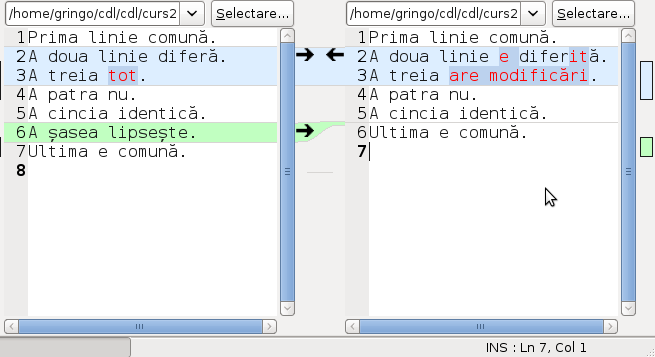
\includegraphics[height=5cm]{code/screenshot-meld.png}%
  \end{itemize}
\end{frame}

\begin{frame}{Un alt mod de a vizualiza diferențele : MELD}
  \begin{itemize}[<+->]
  \item nu ar fi mai ușor de urmărit dacă am avea fișierele de comparat unul lângă altul?
  \end{itemize}
\end{frame}


\begin{frame}[allowframebreaks] % Spargem paginile mai mari automat
% Atenţie: allowframebreaks nu funcţionează cu overlay-uri
\frametitle{Câte ceva despre istoria FLOSS}
\begin{itemize}
\item Punctul de plecare: noua imprimantă de la MIT
\item Proiectul GNU, activismul lui Richard Stallman (1983)
\item Cele patru drepturi. Programele libere nu sunt neapărat gratuite
\item Minix, sistem de operare UNIX educațional. Micronucleu (1987)
\item GNU: un sistem de operare liber dar incomplet. Hurd nu este gata (1990)
\item Linux: nucleul monolitic devenit liber (1991). Primele distribuții
GNU/Linux
\item Afaceri. Companiile multinaționale devin și ele contribuitori la
programele libere
\item OSI și definiția Open Source (1998). Diferențe de perspectivă și
aplicabilitate
\item Patentele pe programe din SUA amenință programele libere. Procese (2004
- prezent)
\item Microsot, Adobe și Nokia încep să dezvolte programe Open Source, nu
toate libere (2008)
\item Echipa Debian se alătură efortului internațional de a termina
revoluționarul GNU Hurd
\end{itemize}
\end{frame}

\section{Cod}
\frame{\tableofcontents[currentsection]}

\begin{frame}
\frametitle{Exemplu de cod}
Acesta este un script bash:\\
\noindent
\ttfamily
\hlstd{}\hlline{\ \ \ \ 1\ }\hlslc{\#!/bin/bash}\\
\hlline{\ \ \ \ 2\ }\hlstd{\\
\hlline{\ \ \ \ 3\ }MAX}\hlsym{=}\hlstd{}\hlnum{10}\\
\hlline{\ \ \ \ 4\ }\hlstd{}\\
\hlline{\ \ \ \ 5\ }\hlkwa{for\ }\hlstd{i\ }\hlkwa{in\ }\hlstd{\$}\hlsym{(}\hlstd{}\hlkwc{seq\ }\hlstd{}\hlnum{1\ }\hlstd{}\hlkwd{\$\{MAX\}}\hlstd{}\hlsym{);\ }\hlstd{}\hlkwa{do}\\
\hlline{\ \ \ \ 6\ }\hlstd{}\hlstd{\ \ \ \ \ \ \ \ }\hlstd{}\hlkwb{echo\ }\hlstd{}\hlstr{"Testing\ \$\{i\}"}\hlstd{}\\
\hlline{\ \ \ \ 7\ }\hlkwa{done}\\
\hlline{\ \ \ \ 8\ }\hlstd{}\\
\hlline{\ \ \ \ 9\ }\hlkwb{exit\ }\hlstd{}\hlnum{0}\hlstd{}\\
\mbox{}
\normalfont
 % includem codul
\end{frame}

\begin{frame}{Încă un exemplu de cod}
Acesta este un program C:

\noindent
\ttfamily
\hlstd{}\hlline{\ \ \ \ 1\ }\hldir{\#include\ $<$stdio.h$>$}\\
\hlline{\ \ \ \ 2\ }\hlstd{}\hldir{\#include\ $<$stdlib.h$>$}\\
\hlline{\ \ \ \ 3\ }\hlstd{}\\
\hlline{\ \ \ \ 4\ }\hldir{\#define\ WHATEVER\ 1}\\
\hlline{\ \ \ \ 5\ }\hlstd{}\\
\hlline{\ \ \ \ 6\ }\hlkwb{int}\\
\hlline{\ \ \ \ 7\ }\hlstd{}\hlkwd{main}\hlstd{}\hlsym{(}\hlstd{}\hlkwb{int\ }\hlstd{argc}\hlsym{,\ }\hlstd{}\hlkwb{char\ }\hlstd{}\hlsym{{*}{*}}\hlstd{argv}\hlsym{)}\\
\hlline{\ \ \ \ 8\ }\hlstd{}\hlsym{\{}\\
\hlline{\ \ \ \ 9\ }\hlstd{}\hlstd{\ \ \ \ \ \ \ \ }\hlstd{}\hlkwd{puts}\hlstd{}\hlsym{(}\hlstd{}\hlstr{"Hello,\ World!}\hlesc{$\backslash$n}\hlstr{"}\hlstd{}\hlsym{);}\\
\hlline{\ \ \ 10\ }\hlstd{\\
\hlline{\ \ \ 11\ }}\hlstd{\ \ \ \ \ \ \ \ }\hlstd{}\hlkwa{return\ }\hlstd{}\hlnum{0}\hlstd{}\hlsym{;}\\
\hlline{\ \ \ 12\ }\hlstd{}\hlsym{\}}\hlstd{}\\
\mbox{}
\normalfont

\end{frame}

\section{Overlay-uri}
\frame{\tableofcontents[currentsection]}

\begin{frame}{Comanda `pause'}
`Pause' ne lasă să arătăm textul `gradual'.

\pause Putem să folosim pause cu itemize sau orice altă facilitate.
\begin{itemize}
\pause \item De exemplu.
\pause \item Încă un exemplu.
\pause \item Dar nu e foarte flexibil...
\end{itemize}
\end{frame}

\begin{frame}{Overlay-uri mai avansate}
\only<1>{Cue chapter 9.3 from the Beamer manual.}
\only<2>{Facem o mare ciorbă de overlay-uri. \textbf{Notă:} E vorba de un
singur slide -- numărul şi titlul se păstrează.}
\begin{itemize}
\item<3-> orice comandă poate fi urmată (fără spaţiu) de un specificator de
overlay;
\item<4-> specificatoarele sunt marcate cu \texttt{<} şi \texttt{>};
\item<5-> \texttt{<4>} înseamnă ``doar pe overlay-ul 4'';
\item<5-> \texttt{<1-3>} înseamnă ``doar pe overlay-urile de la 1 până la 3,
inclusiv'';
\item<6-> \texttt{<5->} înseamnă ``de la overlay-ul 5 până la sfârşit'' (de
fapt, până la slide-ul următor, fireşte);
\item<6-> \texttt{<-4>} înseamnă ``de la început până la overlay-ul 4'';
\item<7-> Toate exemplele de mai sus au avut comanda \texttt{item} urmată de
un overlay. Trebuie să ţinem cont de ordine manual, dar nu cred că vom avea
nevoie de cine-ştie-ce efecte.
\end{itemize}
\end{frame}


\end{document}
